

\section{Cross-section Measurement}
\label{sec:measurement}
\newcommand*\Diff[1]{\mathop{}\!\mathrm{d}#1~}
\newcommand{\boldtheta}{\boldsymbol{\theta}}
\newcommand{\thetas}{\boldsymbol{\theta}_s}
\newcommand{\thetab}{\boldsymbol{\theta}_b}

In this analysis we seek to measure the 
fiducial cross-section, $\sigma^{\textrm{Observed}}$, for the 
WWW production process in the fully-leptonic channel (e,$\mu$).
The observed cross-section is parameterized by looking at the signal
strength, $\mu$, which is related to the expected fiducial cross-sections
from section~\ref{sec:inputs} by the relation:
\begin{equation}
\sigma^{\textrm{Observed}} = \mu \sum_{i\in \textrm{Channels}} \sigma^{\textrm{Fiducial}}_i
\end{equation}

Assuming a counting experiment in each bin $i$, the expected 
event count is given by:
% assuming a simple Poisson counting experiment with expectation for a given bin/channel, $i$:
\begin{align}
%N^{\mathrm{exp}}(\mu,\boldtheta) = N^{\mathrm{exp}}(\mu,\curlyl_0,\Delta_{\curlyl},\thetas,\thetab) = \mu \sum_i \curlyl(\curlyl_0,\Delta_{\curlyl}) \cdot \sigma^{\mathrm{Fiducial}}_i \cdot \varepsilon_i(\thetas) + \sum_{i}\sum_{\mathrm{bkg}} N_{i}^{\mathrm{bkg}}(\thetab)
N^{\mathrm{exp}}_i(\mu,\boldtheta) &= N^{\mathrm{exp}}_i(\mu,\curlyl_0,\Delta_{\curlyl},\thetas,\thetab) \\
 &= \mu \cdot \bigg( \curlyl(\curlyl_0,\Delta_{\curlyl}) \cdot \sigma^{\mathrm{Fiducial}}_i \cdot C_i(\thetas) \bigg) + \sum_{\mathrm{bkg}} N_{i}^{\mathrm{bkg}}(\thetab)
\label{eq:poisson_expectation}
\end{align}
where $C_i$ is the correction factor 
measured in each bin as discussed in section~\ref{sec:inputs} and 
$\sigma^{\mathrm{Fiducial}}_i$ is the fiducial cross-section in each 
bin. The 
individual background expectations in a given bin/channel, $i$, are 
expressed simply by the number of events
for a given background as $N^{\mathrm{bkg}}_i$. 
The signal efficiencies and background expectations are assumed to follow 
probability distributions described by shape parameters determined from 
dedicated measurements of the background normalizations and systematic 
uncertainties.  
The set of correction factor shape parameters are referred to 
as $\thetas$; the set of normalization and shape parameters on 
the background expectations are referred to as $\thetab$.
The integrated luminosity, $\curlyl$, is assumed to have an uncertainty
that follows 
a Gaussian distribution with nominal integrated 
luminosity, $\curlyl_0$, and width, $\Delta_{\curlyl}$. 
Collectively, we refer to all of these parameters, except 
for $\mu$ as the set of nuisance 
parameters, $\boldtheta = (\curlyl_0,\Delta_{\curlyl}, \thetas, \thetab)$. 

The discovery significance is tested using frequentist statistics
to estimate the degree of compatibility with the background-only 
hypothesis~\cite{Cowan:1277304}.
The measurement and uncertainty are evaluated 
by using the shape of the profile likelihood ratio~\cite{PDG:2014} 
which is a function of the data and the signal strength.

\subsection{Profile Likelihood Ratio}

The likelihood used is constructed as follows:
\begin{equation}
L(\mu,\boldtheta) = \mathrm{Gaus}(\curlyl;\curlyl_0,\Delta_{\curlyl})~\prod_{i\in\mathrm{Chan}} \mathrm{Pois}(N_i^{obs}|N_i^{exp}(\mu,\boldtheta))~\prod_{j\in\mathrm{Sys}} \mathrm{Gaus}(\theta_j;\theta_j^0,1)
\label{eq:poisson_likelihood}
\end{equation}
using the HistFactory tool \cite{Cranmer:1456844}. 
Note that the systematic uncertainties are given Gaussian 
constraints with $\pm1\sigma$ uncertainties.

The basic form of the 
test statistic used for comparing hypotheses is called the profile likelihood 
ratio, $\lambda(\mu)$, and is defined as:
\begin{equation}
-\ln \lambda(\mu) = - \ln \frac{L(\mu,\hat{\hat{\boldsymbol{\theta}}}(\mu))}{L(\hat{\mu},\hat{\boldsymbol{\theta}})}
\label{eq:profile_likelihood_ratio}
\end{equation}
Note that it no longer depends on the nuisance parameters, $\boldsymbol{\theta}$,
and instead depends only on $\mu$. 
The denominator is the 
unconditional maximum likelihood (ML)
evaluated at the ML estimators $\hat{\mu}$ and $\hat{\boldsymbol{\theta}}$.
This quantity is a unique constant when specified for a given likelihood
and set of nuisance parameters.
The numerator is the conditional ML which depends on $\mu$ and
evaluated at 
the conditional ML estimator for the set of nuisance parameters, 
$\hat{\hat{\boldsymbol{\theta}}}$, which itself depends on $\mu$.
The presence of the nuisance parameters are handled in the profiling 
step when constructing the profile likelihood ratio,  which results 
in a smearing of the profile likelihood ratio contour. 
During profiling, the systematic uncertainties are
interpolated using a piecewise linear function for shape uncertainties
and a piecewise exponential function for the normalization uncertainties
in order to maintain a normalization that is greater than zero.
The negative of the logarithm of the profile likelihood 
ratio is used because
the logarithm is monotonic and typically easier to work with.
Clearly, the profile likelihood ratio runs from $0 < \lambda(\mu) < 1$
with values close to $0$ showing more agreement with the background 
only hypothesis and values closer to $1$ showing more agreement with 
the signal hypothesis.
When taking the negative log likelihood, the range
is mapped to the entire positive axis and inverted. This means
that values close to $0$ are more background-like and larger values 
are more signal-like.  

The minimum of the negative log of the profile likelihood 
is taken as the measurement of the signal strength; 
the uncertainty on the measurement is taken from the shape of the 
negative log profile likelihood assuming the behavior in the asymptotic
limit can be used.  The asymptotic behavior of the profile likelihood 
is used to evaluate the final confidence interval. 


\subsection{Testing for Discovery Significance}
The rejection of the background-only hypothesis ($\mu = 0$) is used 
to estimate the significance of a possible observation of the signal.
For the purposes of this test, the following test 
statistic is used:
\begin{equation}
q_{0} = 
\begin{cases}
\hfill -2 \ln \lambda(0),\hfill & \hat{\mu} \geq 0 \\
0,\hfill & \hat{\mu} < 0
\end{cases}
\label{eq:q0}
\end{equation}
The test statistic is set to $0$ when $\hat{\mu} < 0$ to enforce
the notion that an observation which is less than the background
expectation should not be treated as signal like. The $p$-value in this case
tells us the degree of incompatibility with the background-only hypothesis
and is defined as:
\begin{equation}
p_0=\int^{\infty }_{q_{0,\textrm{obs}}} f(q_0|\mu=0) \Diff{q_0}
\label{eq:pvalue}
\end{equation}
where $q_{0,\textrm{obs}}$ is the observed value of $q_0$ and 
$f(q_0|\mu=0)$ is the probability density of the test statistic $q_0$ under
the background-only hypothesis which is evaluated using MC. %explain?
By examining the $p$-value one can say what the probability is 
that the deviation away from the background-only hypothesis is due
to chance. A small probability suggests that such a fluctuation is
unlikely. Frequently one refers to the significance:
\begin{equation}
Z = \Phi^{-1}(1-p_0)
\label{eq:significance}
\end{equation}
where $\Phi^{-1}$ is the inverse of the Gaussian cumulative distribution 
function.
In this way, one may refer to $Z\sigma$ significance of a measurement 
where usually
$3\sigma$ is considered to constitute 'evidence' and $5\sigma$ constitutes
discovery.

The distribution of $q_0$ is 
shown in Fig.~\ref{fig:stat_measurement_significance} for the combination.  
The observed null p-value 
is found to be 0.24 for the combination which corresponds to a significance
of $0.70 \sigma$.  One may compare to this to an expected 
p-value of 0.25 corresponding to 
a significance of $0.66 \sigma$.

\begin{figure}[ht!]
\centering
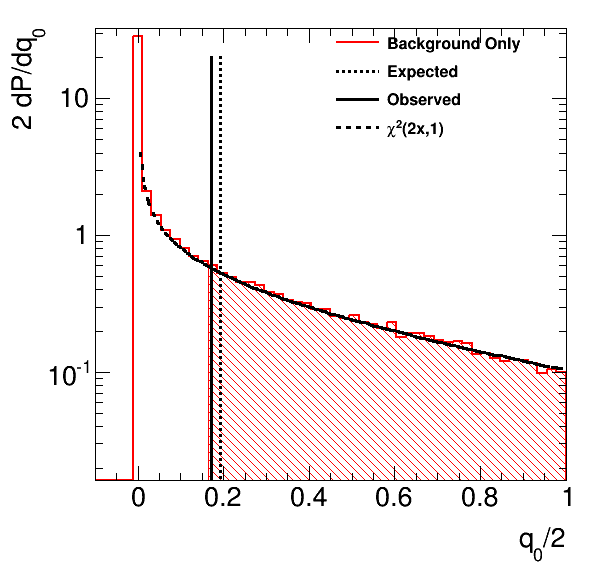
\includegraphics[width=0.50\columnwidth]{figures/statistics/significance/combination.png}
\caption{Probability distribution of the background-only hypothesis as a function of $q_0$ for 
the combination of all three channels. The probability distributions are determined 
using toy MC. The solid black line represents the observed 
value of $q_0$ seen in the data. The shaded area above
this line represents the null p-value or the 
integral of the background hypothesis in the signal-like region.
The dotted black curve shows a $\chi^2$ distribution for 1 degree of 
freedom with which 
it can be seen is a good approximation of the 
the background-only PDF.}
\label{fig:stat_measurement_significance}
\end{figure}


\subsection{Measurement and Uncertainty using Profile Likelihood Interval}

The measured value of the signal strength is determined by looking 
at the minimum 
of the negative log profile likelihood for each channel separately and also 
for the combination of all channels. The size of the uncertainty on the 
measurement is taken by looking at the shape of the negative log 
profile likelihood contour which in general should follow a parabolic
shape centered about the minimum in the asymptotic limit. In this limit,
Wilk's theorem \cite{Wilk:1938}
can be used \cite{PDG:2014}
to determine that
the range of the 
uncertainty for a given number of Gaussian $\sigma$ can be related
directly 
to the negative profile log likelihood.  In particular, for 
a $1\sigma$ uncertainty one expects that 
$|-\ln \lambda(\mu)| \leq 1/2$.
%\begin{equation}
%-2 \ln \lambda(\mu) = s^2
%\end{equation}
Note that even if the contour is not distributed symmetrically about 
the minimum
value, invariance of the likelihood under 
transformations like $g(\hat{\mu},\hat{\boldsymbol{\theta}})$ where $g$ is some function, 
means the same conclusion still holds.
The range of the measured value of $\mu$ is left unrestricted and thus
allowed to become negative.

The profile likelihood contour is evaluated once without 
systematic uncertainties included
as nuisance parameters in order to estimate the size of the 
measurement uncertainty purely 
from statistical effects. It is then then evaluated a second time with the 
systematic uncertainties included
as nuisance parameters whose errors are constrained to be Gaussian and then 
profiled out. The contour with systematic uncertainties included represents
the total uncertainty. The systematic uncertainty is determined by 
assuming that
the total uncertainty is formed from the statistical and systematic 
uncertainties being added
in quadrature.
%The negative log likelihood contours as well as their uncertainties are shown for the individual channels in
%Fig.~\ref{fig:stat_measurement_interval_channels} 
The negative log likelihood contour is 
for the combination of all three channels in 
Fig.~\ref{fig:stat_measurement_interval_combination}.
The expected value and uncertainties for the fiducial cross-section is:
\begin{equation}
\sigma^{\textrm{Expected}} = 309.2  ^{+434}_{-338} (\textrm{stat}) ^{+316}_{-342} (\textrm{sys}) \textrm{ab}
\end{equation}
and the observed fiducial cross-section is:
\begin{equation}
\sigma^{\textrm{Observed:}} = 315.1  ^{+347}_{-334} (\textrm{stat}) ^{+326}_{-348} (\textrm{sys}) \textrm{ab}
\end{equation}

%\begin{figure}[ht!]
%\centering
%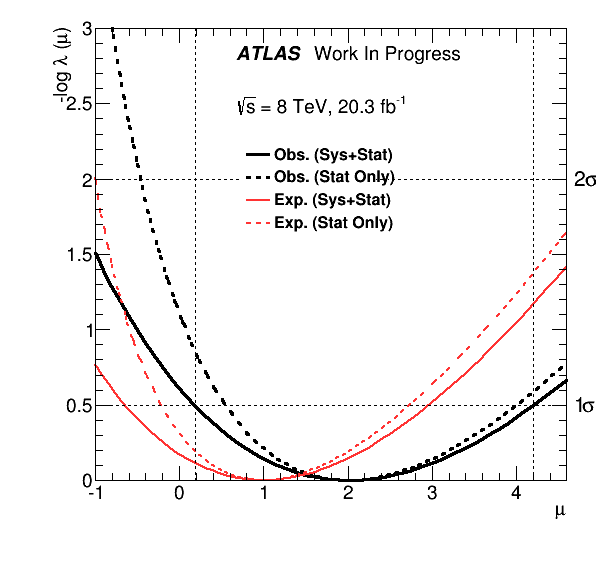
\includegraphics[scale=0.25]{figures/statistics/measurement/interval/0sfos.png}
%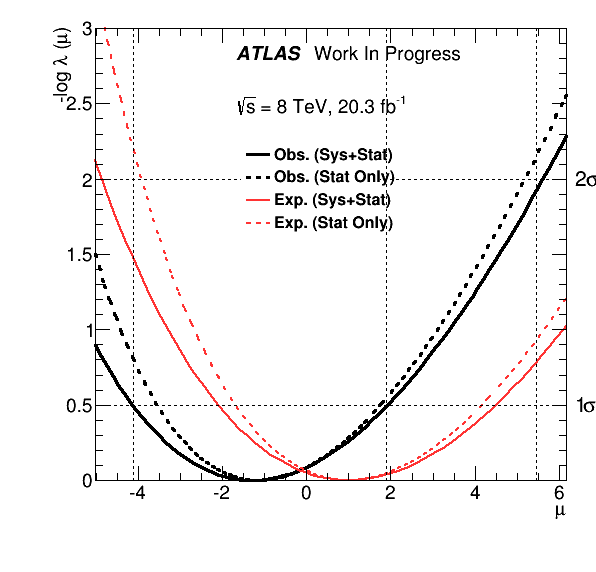
\includegraphics[scale=0.25]{figures/statistics/measurement/interval/1sfos.png}
%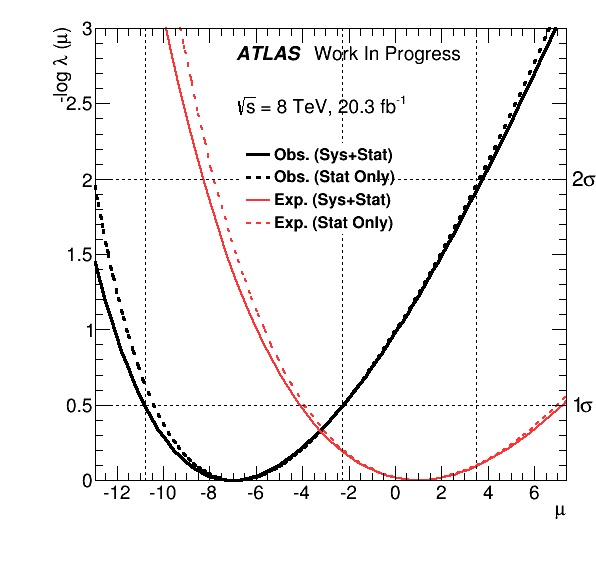
\includegraphics[scale=0.25]{figures/statistics/measurement/interval/2sfos.png}
%\caption{The profile likelihood contours evaluated as a function of the signal strength for the 0 SFOS (left), 1 SFOS (middle), and 2 SFOS (right) channels. The observed (black) and expected (red) contours are shown when considering only statistical uncertainty (dashed line) and when considering both statistical and systematic uncertainties (solid line).  The dotted black lines pinpoint the location of the $1~\sigma$ and $2~\sigma$ total Gaussian uncertainties on the measurement of the signal strength which corresponds to the minimum value of the contour.}
%\label{fig:stat_measurement_interval_channels}
%\end{figure}

\begin{figure}[ht!]
\centering
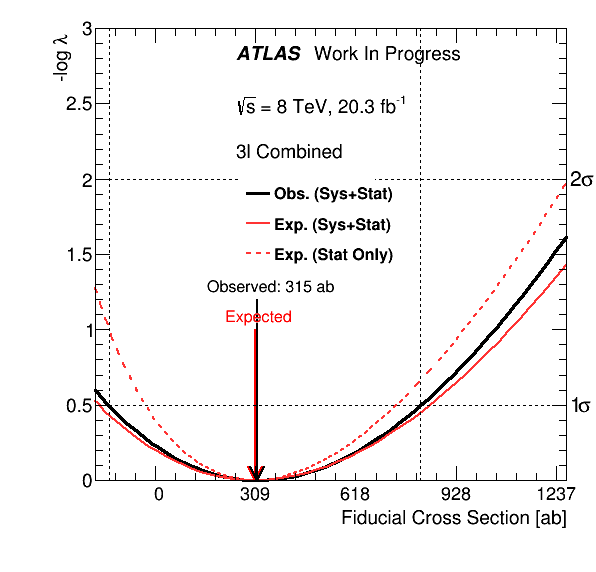
\includegraphics[scale=0.5]{figures/statistics/measurement/interval/combination.png}
%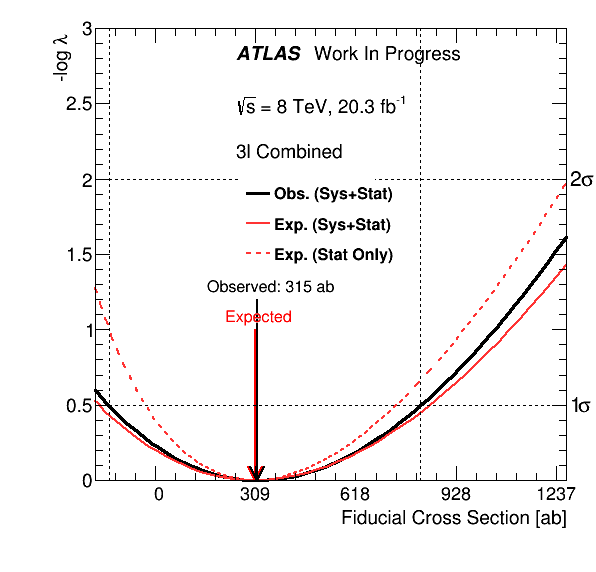
\includegraphics[width=0.8\columnwidth]{figures/statistics/measurement/interval/combination.png}
\caption{The profile likelihood contours evaluated as a function of 
the signal strength
for the combination of all three channels. 
The observed (black) and expected (red) contours are shown when 
considering only statistical uncertainty (dashed line) and when considering both statistical and systematic uncertainties (solid line).
The dotted black
lines pinpoint the location of the $1~\sigma$ and $2~\sigma$ total 
Gaussian uncertainties
on the measurement of the signal strength which corresponds to the 
minimum value of the contour.}
\label{fig:stat_measurement_interval_combination}
\end{figure}


